\section{Herramientas para el desarrollo blockchain}

\subsection{Tipos de redes Blockchain}

Cuando la tecnología Blockchain fue introducida al mundo, era del tipo público en el caso de uso de criptomonedas, pero
con el paso del tiempo y las posibles aplicaciones que se podían llevar a cabo, dió lugar a diferentes casificaciones 
comúnmente aceptadas. Las redes blockchain se pueden clasificar entre públicas o privadas, y dos modos diferentes: 
abiertas o cerradas. Dando el resultado de cuatro posibles configuraciones.

\vspace{5mm}

\noindent La comparación de estos dos últimos va asociado a quién es capaz de leer esos datos de la Blockchain Y así, 
podemos hablar de soluciones que son públicas y abiertas, públicas y cerradas, privadas y abiertas, privadas y 
cerradas.

\vspace{5mm}

\noindent Un ejemplo se puede ver a continuación en la siguiente figura (ver fig.\ref{fig:tipos-de-redes}):

\vspace{5mm}

\begin{figure}[ht!]
    \centering
    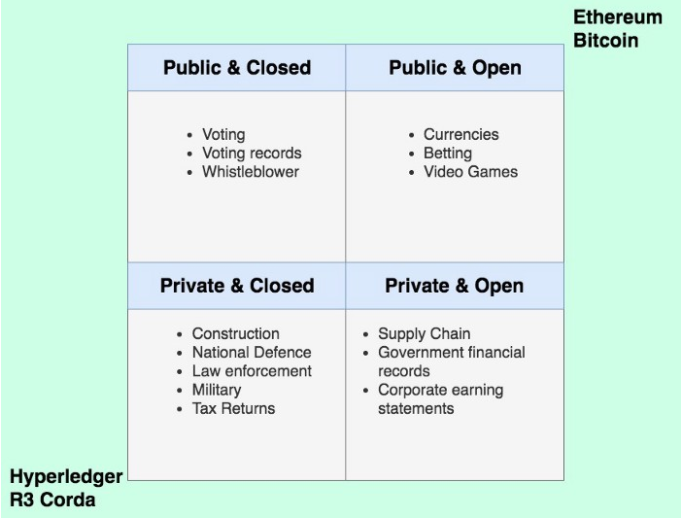
\includegraphics[width=10cm]{imagenes/herramientas/tipos_de_redes}
    \caption{Tipos de redes con sus posibles aplicaciones}
    \label{fig:tipos-de-redes}
\end{figure}

\vspace{5mm}

\noindent En esta sección vamos a definir los diferentes tipos de redes y sus posibles prácticas.

\subsubsection*{Redes públicas (permissionless)}

Cuando hablamos de redes públicas (permissionless), nos referimos a redes públicas abiertas. Es un Blockchain que 
permite que cualquiera pueda unirse a la red, lo que significa que puede leer, escribir o participar en ella. Las 
Blockchain públicas están descentralizadas, nadie tiene control sobre la red, y están seguras de que los datos no 
pueden ser cambiados una vez validados. Este tipo de Blockchain tiende a centrarse más en un escenario B2C o
Business to Customer.

\vspace{5mm}

\noindent Las plataformas que podemos encontrar son Bitcoin, Ethereum entre otras criptomonedas. Al no haber permisos,
este tipo de redes se centran en proteger el anonimato de los usuarios y por tanto, no se pueden establecer roles y
controles en qué datos se pueden leer o escribir.

\subsubsection*{Redes privadas (permissioned)}

En contraparte, las redes Blockchain privadas son del tipo cerradas, ya que queremos controlar quien escribe y lee los 
datos de la Blockchain, y por ende tenemos que establecer entidades. Se definen reglas sobre qué datos pueden añadir al 
libro mayor y qué datos pueden consumir del libro mayor. La mayoría de veces, vienen incorporados con herramientas de 
gestión de identidades (OAuth). 

\vspace{5mm}

\noindent Las Blockchain privadas también son conocidas como Enterprise Blockchains, ya que son las más utilizadas por 
empresas. Pueden ser Open Source, de consorcio o desarrolladas de forma privada. Las opciones más comunes son 
Hyperledger, R3 Corda y Quorum. Por esta razón, están estructuradas a un modelo B2B o Business to Business. 

\vspace{5mm}

\noindent Las transacciones son procesadas por una cantidad mínina y conocida de nodos de la Blockchain, en comparación 
con las redes públicas, como los 8000 nodos en el caso de Ethereum. Hay una clara diferencia en rendimiento entorno a 
la latencia y velocidades de transmisión.

\subsubsection*{Beneficios de una red pública}

\begin{itemize}
\item \textbf{Abierto a lectura y/o escritura}: Cualquiera puede participar enviando transacciones al Blockchain, como 
Ethereum o Bitcoin; las transacciones pueden verse en el explorador del Blockchain.

\item \textbf{El libro mayor es distribuido}: No está centralizado como en un enfoque cliente-servidor, y todos los 
nodos participan en la validación de la transacción.

\item \textbf{Inmutable}.

\item \textbf{Seguro gracias a la minería (regla del 51\%)}: Por ejemplo, con Bitcoin, la obtención de la mayor parte 
de la potencia de la red podría permitir una duplicación masiva de los gastos, y la posibilidad de evitar 
confirmaciones de transacciones, entre otros actos potencialmente malintencionados.
\end{itemize}

\subsubsection*{Beneficios de una red privada}

\begin{itemize}
\item \textbf{Permisos empresariales}: La empresa controla los recursos y el acceso, por lo tanto, es privada y/o 
autorizada.

\item \textbf{Transacciones más rápidas}: Cuando distribuyes los nodos localmente, y también tienes muchos menos nodos 
participantes, el rendimiento es más rápido.

\item \textbf{Mejor escalabilidad}: El hecho de poder añadir nodos y servicios a petición puede ser una gran ventaja 
para la empresa.

\item \textbf{Soporte de cumplimiento}: Como empresa, tiene que satisfacer con requisitos de cumplimiento, y tener el 
control de su infraestructura, esto permite que se cumpla más fácilmente.

\item \textbf{Consenso más eficiente (menos nodos)}: Las Blockchain empresariales o privadas tienen menos nodos y 
suelen tener un algoritmo de consenso diferente, como BFT vs PoW.
\end{itemize}

\subsection{Plataformas Blockchain}

Conocemos de antemano, que la tecnología Blockchain surgió en 2008 con la plataforma Bitcoin, y ha evolucionado hasta
convertirse en una tecnología dominante, utilizada también a nivel empresarial, y por tanto han surgido nuevas y 
diversas plataformas de Blockchain. En la sección anterior, hemos comentado algunas plataformas, según su tipo de red,
es el momento de dar paso a definir la lista de las plataformas más conocidas de Blockchain que hay actualmente.

\subsubsection{Plataformas de Blockchain populares}

\subsubsection*{Hyperledger}

Hyperledger es conocidad por ser una de las mejores plataformas blockchain de Open-source. Está alojada por la Linux 
Fundation y permite a los usuarios crear y desarrollar frameworks distribuidos de libro de contabilidad a nivel 
empresarial. Se creó en 2015 y hay una amplia gama de frameworks dirigidos a diferentes casos de uso. Cabe mencionar
los siguientes: 
    
\begin{itemize}
    \item \textbf{Hyperledger Fabric}: es un framework de Blockchain para las empresas. Ofrece una amplia gama de 
    características, incluyendo servicios de membresía y consenso. Además, también puede alojar contratos inteligentes 
    llamados \say{chaincode}. IBM y Digital Asses son los primeros en contribuir al proyecto.
    \item \textbf{Hyperledger Sawtooth}: es una plataforma modular, diseñadad para desplegar y ejecutar DLT sin una
    autoridad central.
    \item \textbf{Hyperledger Iroha}: es una plataforma de cadena de bloques para la construcción de aplicaciones 
    descentralizadas confiables, seguras y rápidas.
\end{itemize}

\vspace{5mm}

\noindent Este tipo de plataforma es permissioned, por tanto la entrada a la red de un nuevo participante ha de ser
aprobada por el resto de nodos, se crean canales de comunicación, donde se implementan la privacidad de transacciones.
Se puede catalogar como subredes dentro de la propia red.

\subsubsection*{R3 Corda}

R3 Corda es una plataforma de cadena de bloques de código abierto. Es una tecnología de libro mayor distribuido.

\vspace{5mm}

\noindent Su enfoque es bastante diferente de la cadena de bloques tradicional, donde una transacción necesita ser 
verificada por muchos nodos. Su enfoque es reducir el número de validaciones y mejorar la eficiencia mientras se 
mantiene intacto todo el conjunto de características de la cadena de bloques.

\vspace{5mm}

\noindent Las tres características clave de R3 Corda son el código abierto, el diseño abierto y el desarrollo abierto. 
Esto significa que cualquiera puede usar R3 Corda y utilizar la plataforma de cadena de bloques de código abierto 
según sus necesidades y requerimientos. 

\subsubsection*{Ethereum}

Ethereum es una de las plataformas blockchain más importantes, destacamos de ella ser pionera en los Smart contract así 
como la ejecución simple de los mismos. Creada por Vitalk Buterin en 2013 y es una plataforma de código abierto y 
pública. Su moneda es el Ether. Sigue un mecanismo de consenso PoW, que es comparativamente más lento en velocidad, 
pero van a modificar el algoritmo a prueba de participación o Proof-of-Stake\footnote{Proof-of-Stake (PoS) establece 
que una persona puede minar o validar transacciones dependiendo de la cantidad de monedas que tenga. Esto significa que 
cuantas más monedas posea un minero, más poder de mineria tendrá.\label{fnlabel}}.

\vspace{5mm}

\noindent Ethereum tiene, también, un apartado para empresas conocido como Enterprise Ethereum. Ofrece una cadena de 
bloqueo flexible, segura y escalable dirigida a los negocios. Ofrece tres tipos de implementación, incluyendo privada, 
híbrida y de consorcio. Esto significa que cualquier empresa puede aprovechar las ventajas del Ethereum adaptándolo a 
sus necesidades. Con las herramientas proporcionadas, puede crear aplicaciones descentralizadas (dApp\footnote{
Aplicación software que está construida en una red descentralizada.\label{fnlabel}}). 

\subsubsection*{Quorum}

Quorum es una plataforma de código abierto diseñada para mejorar la privacidad. Es una innovación basada en Ethereum, 
desarrollada en asociación con J.P. Morgan y EthLab, una startup de Ethereum. Modifica el núcleo de Ethereum y, por lo 
tanto, tiene muchas más características excepcionales añadidas que la tecnología tradicional de cadenas de bloques.

\vspace{5mm}

\noindent Esta plataforma permite implementaciones de consensos diferentes según las necesidades. Ofrece privacidad a 
nivel de transacción, junto con transparencia en toda la red, y no soporta la política global de intercambio de datos. 
Actualmente, la platforma de Quórum se está convirtiendo en una parte indispensable de organizaciones como bancos e 
instituciones financieras en las que la privacidad de los datos es crucial.

\subsubsection*{Ripple}

Es una plataforma de cadena de bloques de código abierto que está diseñada para permitir transacciones rápidas y 
baratas. Su criptodivisa es conocida como XRP, pero también permite a la gente crear su propia moneda a través de 
RippleNet. RippleNet permite a los usuarios encontrar nuevos clientes en nuevos mercados, ampliar los servicios y 
ofrecer la mejor experiencia en pagos globales. A diferencia de los métodos de transacción tradicionales, esta 
plataforma tiene por objeto facilitar y agilizar el proceso de transacción, especialmente en el caso de los pagos 
transfronterizos, creando así un mejor ecosistema de crecimiento y desarrollo.

\subsubsection{Blockchain como plataformas de servico (BaaS)}

Blockchain-as-a-Service o BaaS, es la creación y gestión por parte de terceros de redes basadas en la nube para 
empresas que se dedican a la construcción de aplicaciones Blockchain. Estos servicios de terceros son un desarrollo 
relativamente nuevo en el creciente campo de la tecnología de las Blockchain, El negocio de la tecnología ha superado 
con creces su uso más conocido en las transacciones en criptografía y se ha ampliado para abordar las transacciones 
seguras de todo tipo. Las empresas basadas en la nube que implementan la tecnología Blockchain tenemos:

\subsubsection*{IBM}

IBM es la empresa pionera en aventurarse en la creación de una plataforma Blockchain para operaciones comerciales
transparentes. Posee unaa división encargada de crear aplicaciones basada en Blockchain.

\vspace{5mm}

\noindent Ofrece una red permissioned, y asegura a las empresas que puedan construir, digirir, operar y crecer usando
la tecnologia de IBM. Soporta Golang y Java.

\subsubsection*{Amazon}

Amazon también ofrece su solución BaaS con el uso de Amazon Managed Blockchain. Con él, puedes crear y gestionar la 
Blockchain. Funciona con redes de cadenas de bloques populares como Ethereum y Hyperledger Fabric.

\vspace{5mm}

\noindent Tiene los siguientes beneficios:

\begin{itemize}
    \item Completamente administrado
    \item Se puede escoger entre Ethereum o Hyperledger Fabric
    \item Seguro y escalable
    \item Confiable
\end{itemize}

\vspace{5mm}

\noindent Ofrece una amplia gama de soluciones, incluyendo Amazon QLDB (Quatum Ledger Database), Amazon Manaaged 
Blockchain, AWS Blockchain Templates, y AWS Blockchain Partners.

\subsubsection{Otras plataformas Blockchain}

\subsubsection*{OpenChain}

Es de código abierto y se dirige principalmente a organizaciones que quieren asegurarse de que sus activos digitales
se gestionan y emiten de forma seguro, robusta y escalable.

\vspace{5mm}

\noindent Es fácil de usar y administrar, pudiendo establecer reglas para los usuarios finales que participen e 
intercambien el valor definido por esas reglas. Cada transacción está firmada digitalmente para garantizar la 
seguridad. Utiliza el consenso particionado. Cada instancia de Openchain tiene una autoridad para la validez de 
la transacción, en la que la Blockchain utiliza las instancias de Openchain con fines de descentralización. Esto 
significa que la transacción debe ser validada por diferentes instancias de OpenChain.

\vspace{5mm}

\noindent Otras características fundamentales de OpenChain son una mayor eficiencia gracias al uso de una arquitectura 
cliente-servidor y la ausencia de minadores. Esto también significa que las transacciones no necesitan ningún 
tipo de tasas y son instantáneas.

\subsubsection*{Stellar}

Stellar es un libro de contabilidad distribuido basado en cadenas de bloques que se utiliza para facilitar las 
transferencias cruzadas de valor. De manera similar a Ripple, también puede tratar con intercambios entre criptodivisas. 
Es posible construir herramientas bancarias, dispositivos inteligentes y carteras móviles utilizando la red Stellar.


\vspace{5mm}

\noindent El Protocolo de Consenso Estelar (SCP) permite llegar a un consenso sin depender de un sistema cerrado de 
registro de las transacciones financieras. Al tener un conjunto de propiedades de seguridad comprobables, el SCP 
optimiza la seguridad sobre la vida deteniendo el progreso de la red hasta que se pueda llegar a un consenso en 
caso de que los nodos o la partición se comporten mal.

\vspace{5mm}

\noindent En comparación con los algoritmos descentralizados de prueba de trabajo y prueba de toma, SCP tiene requisitos 
financieros e informáticos modestos, lo que reduce la barrera de entrada y abre el sistema financiero a nuevos 
participantes.

\subsection{Smart Contracts}

Los contratos inteligentes proporcionan una solución a ese problema exactamente. Pueden formalizar las relaciones entre personas e instituciones y los bienes que poseen a través de Internet, totalmente P2P, sin necesidad de intermediarios de confianza. Aunque el concepto de contratos inteligentes no es nuevo, las tecnologías de cadenas de bloques parecen ser el catalizador para la implementación de contratos inteligentes

Un contrato inteligente es un acuerdo de auto-ejecución incrustado en un código informático gestionado por una cadena de bloqueo. El código contiene un conjunto de reglas bajo las cuales las partes de ese contrato inteligente acuerdan interactuar entre sí. Si se cumplen las reglas predefinidas, el acuerdo se hace cumplir automáticamente. Los contratos inteligentes proporcionan mecanismos para gestionar eficazmente los activos simbólicos y los derechos de acceso entre dos o más partes. 

Los valores y derechos de acceso subyacentes que gestionan se almacenan en una cadena de bloques, que es un libro mayor transparente y compartido, donde están protegidos contra la supresión, la manipulación y la revisión. Los contratos inteligentes, por lo tanto, proporcionan una forma pública y verificable de integrar las reglas de gobierno y la lógica empresarial en unas pocas líneas de código, que pueden ser auditadas y aplicadas por el consenso mayoritario de una red P2P.

Un contrato inteligente puede ser invocado desde entidades dentro (otros contratos inteligentes) y fuera (fuentes de datos externas) de la cadena de bloques. Entre estas entidades, los llamados "oráculos" inyectan datos relevantes para el contrato inteligente desde el mundo de la cadena al almacén de información del contrato inteligente. Si se aplican correctamente, los contratos inteligentes podrían proporcionar una seguridad en las transacciones superior a la del derecho contractual tradicional, con lo que se reducirían los costos de coordinación de la auditoría y el cumplimiento de esos acuerdos. 

\subsubsection*{Casos de uso}

Los casos de uso de contratos inteligentes van de simples a complejos. Pueden utilizarse para transacciones económicas sencillas como el envío de dinero de A a B. Los contratos inteligentes también pueden utilizarse para registrar cualquier tipo de propiedad y de derechos de propiedad, como los registros de tierras y la propiedad intelectual, o para gestionar el control de acceso inteligente para la economía de reparto. Se pueden encontrar casos de uso en la banca, los seguros, la energía, el gobierno electrónico, las telecomunicaciones, la industria musical, el arte, la movilidad, la educación y muchos más.

\subsection{Herramientas utilizadas para Hyperledger Fabric}

\subsection{Herramientas utilizadas para desarrollo del proyecto}

\subsection{Conclusión}

\newpage